\documentclass[runningheads]{llncs}

\usepackage[T1]{fontenc}
\usepackage{graphicx}
\usepackage{booktabs}
\usepackage{amsmath}
\usepackage{amssymb}
\usepackage{marvosym}
\usepackage{url}
\usepackage{placeins}

\newcommand{\method}{SARGE}

\begin{document}

\title{\method: Schema-Grounded Event-Table Generation for Chinese Financial Document-Level Event Extraction}
\titlerunning{\method: Schema-Grounded Event-Table Generation}

\author{Jiakai Tong\inst{1,2}\orcidID{0009-0007-9118-5117} \and
Mengting Qin\inst{1}\orcidID{0009-0008-7447-677X} \and
Yongqi Hu\inst{1} \and
Xueyao Wan\inst{1,2} \and
Yue Zhao\inst{1,2}\orcidID{0000-0002-5970-5844}\,(\Letter)}
\authorrunning{J. Tong et al.}
\institute{School of Astronautics, Harbin Institute of Technology, Harbin 150001, China\\
\email{yue.zhao@hit.edu.cn} \and
Zhengzhou Advanced Research Institute, Harbin Institute of Technology, Zhengzhou 450000, China}

\maketitle

\begin{abstract}
Chinese financial document-level event extraction converts long announcements into fixed-schema event tables. Homogeneous-record binding is difficult: several same-type events may share public arguments, allowing correct role values to be recovered yet still assembled into incorrect rows. This paper presents \method\ (Schema-Aware Role-Grounded Extractor), a contract-centered event-table generator that treats the fixed-slot financial event table as the central prediction object, renders the closed financial event schema as a role-grounded output contract, and instruction-tunes a 4B language model to generate schema-checked fixed-slot event rows. On ChFinAnn and DuEE-Fin, \method\ reaches F1 of 86.0 and 78.0, above the listed baselines on ChFinAnn and, on DuEE-Fin, below SEELE but above EPAL and ProCNet. Its advantage is most pronounced where the task is hardest: on the multi-event subset, where homogeneous records must be assembled from shared evidence, \method\ reaches 81.8 F1(M.) on ChFinAnn, above the strongest reported baselines and with the smallest single-to-multi degradation among comparable systems. Without task-specific tuning the same base model drops to F1 24.8 and 3.3, locating the gain in schema-grounded alignment rather than scale. We further introduce a record-level diagnostic pair, ExactRec and $\Delta_{\mathrm{record}}$, that measures exact event-row assembly beyond F1.
\keywords{Document-level event extraction \and Financial text mining \and Schema-grounded generation \and Event-table generation}
\end{abstract}

\section{Introduction}
\label{sec:introduction}

Chinese financial announcements are a central source of evidence for corporate operations, capital-market activities, and risk disclosures. Document-level event extraction (DEE) converts such announcements into structured event tables by identifying event types and filling predefined roles with participants, monetary values, dates, ratios, share quantities, and counterparties \cite{chen2025docfee,han2022dueefin,zheng2019doc2edag}. Compared with sentence-level extraction, financial DEE must integrate scattered evidence into complete schema-defined records, and record-level success is the operative target.

The defining challenge of this setting is record organization under shared evidence. A single announcement may contain several same-type records that share company names, disclosure dates, transaction objects, or background statements, while their differences appear only in private values such as pledgees, amounts, share quantities, or time spans. A system must therefore recover document-grounded role values and assign them to coherent event rows; otherwise many arguments can be correct while final rows are merged, split, or cross-bound. As Fig.~\ref{fig:binding-gap} illustrates, homogeneous records produce surface similarity in shared public arguments, while the private values that distinguish records may be short, repeated, or distributed across nearby sentences. Chinese financial DEE is thus better viewed as schema-grounded event-table construction from document evidence than as entity detection followed by independent role classification.

Existing systems have made substantial progress with pre-trained encoders and task-specific structured prediction. They use entity candidates, graphs, event queries, proxy nodes, and schema descriptions for cross-sentence and multi-event reasoning \cite{hu2025epal,liang2022raat,wang2023procnet,xu2021git,xu2024seele,yang2021deppn,zheng2019doc2edag,zhu2022ptpcg}. These works establish that schema and role structure are central to financial DEE, and they motivate the same premise as \method. They also distribute document understanding, role semantics, schema constraints, and final table construction across separate modules, leaving an opportunity to make the schema the contract that governs generation, validation, and evaluation.

Closed-schema financial DEE is well suited to schema-grounded generation. Event types and role sets are fixed, and many of these values appear verbatim as source-text strings. The desired output is an event table rather than free-form text, which makes it possible to expose the schema as an output contract while keeping generation tied to document-visible evidence.

\method\ instantiates this view by rendering the schema as a role-grounded output contract, exposing bounded source-value cues, instruction-tuning a language model to generate event rows, decoding deterministically, and applying schema-checked fixed-slot table construction. Document evidence, role selection, schema adherence, and table construction are represented through one event-table interface rather than through separate output spaces.

This paper makes three contributions.
\begin{itemize}
\item We present \method, a contract-centered generative framework that treats the fixed-slot financial event table as the prediction object and renders the closed schema as a role-grounded output contract.
\item We instantiate this formulation as an instruction-tuned LLM: it reaches F1 of 86.0 on ChFinAnn and 78.0 on DuEE-Fin, competitive with specialized discriminative systems, and its value is clearest on the multi-event subset, where it reaches 81.8 F1(M.) on ChFinAnn above the strongest reported baselines and degrades least from single- to multi-event documents.
\item We provide a record-level diagnostic analysis with ExactRec and $\Delta_{\mathrm{record}}$, showing that F1 can hide cross-bound or incomplete event records.
\end{itemize}

The contribution is deliberately conservative: \method\ does not open the event inventory or replace evaluation with free-form generation. Instead, it makes the fixed schema the organizing contract for generation, validation, and evaluation, so that the model outputs benchmark-compatible rows while ExactRec exposes the remaining record-assembly errors.

\begin{figure}[t]
\centering
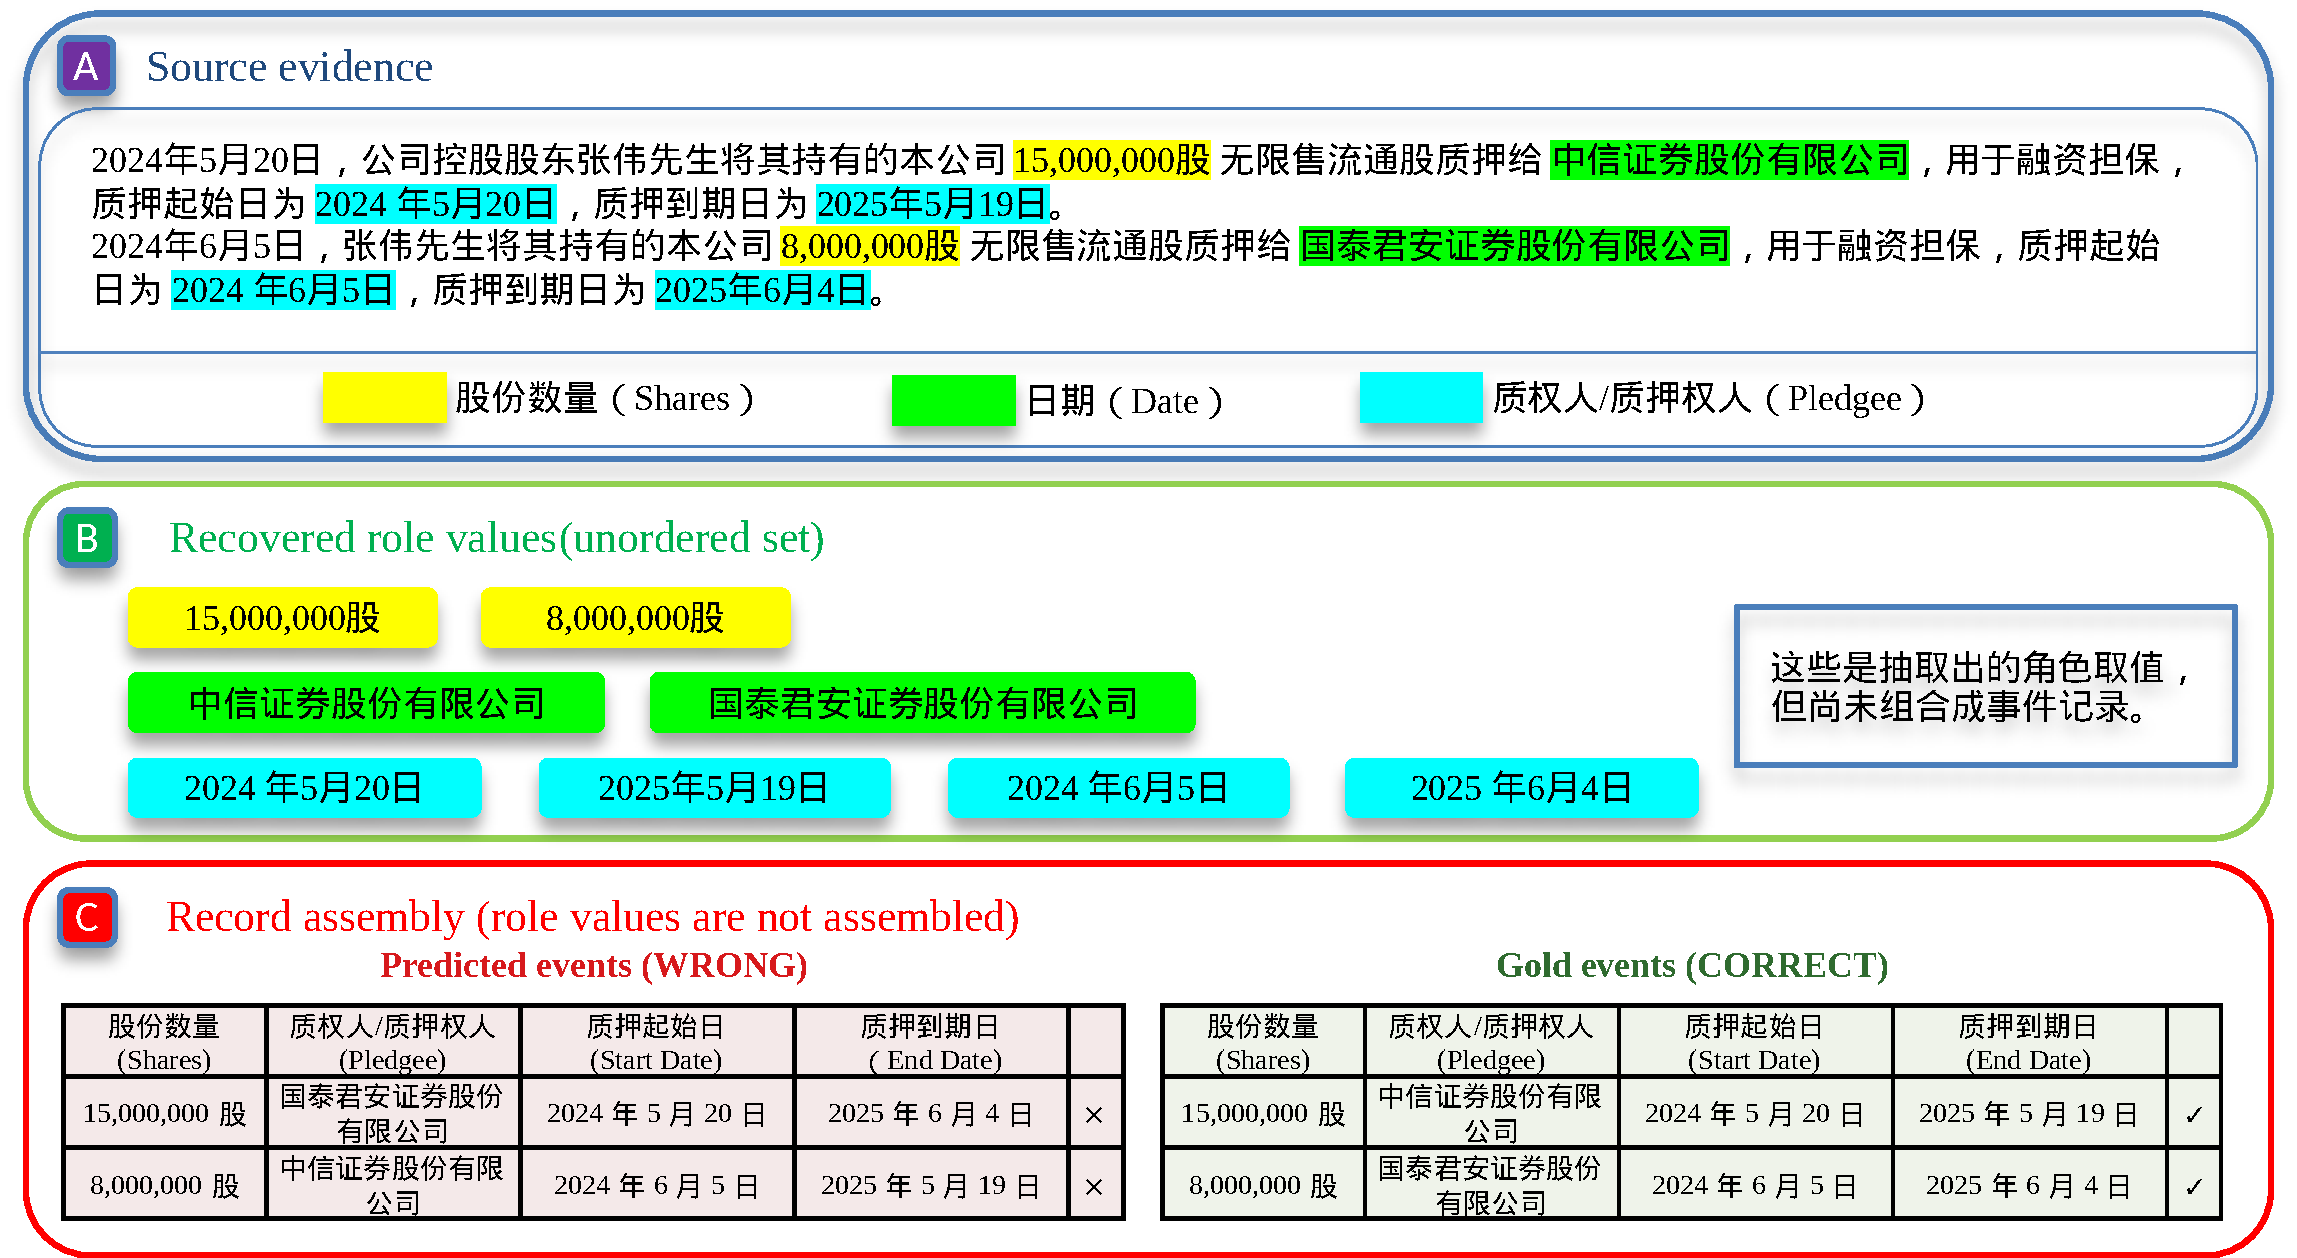
\includegraphics[width=\linewidth]{figures/fig1_binding_gap_ref.pdf}
\caption{Homogeneous-record binding gap in Chinese financial DEE. Even when correct role values are recovered from the source document, private arguments such as pledgee, shares, and date need to be bound into coherent same-type event rows.}
\label{fig:binding-gap}
\end{figure}

\section{Related Work}
\label{sec:related}

Doc2EDAG frames document-level financial event extraction as no-trigger event-table filling and represents Chinese financial announcements as typed fixed-role records \cite{zheng2019doc2edag}. Later encoder, graph, proxy, and pre-filling systems include DE-PPN, GIT, ReDEE/RAAT, PTPCG, ProCNet, IPGPF, and SEELE \cite{huang2023ipgpf,liang2022raat,wang2023procnet,xu2021git,xu2024seele,yang2021deppn,zhu2022ptpcg}; DuEE-Fin and DocFEE broaden the dataset setting \cite{chen2025docfee,han2022dueefin}. EPAL targets homogeneous multi-event extraction with event-specific probes and argument libraries \cite{hu2025epal}. These works share the same premise as \method, namely that schema semantics and record-level role organization are core to financial DEE, while \method\ makes schema roles and source-value selection part of a generative event-table contract rather than an encoder-side objective.

Generation-based information extraction casts structured prediction as text-to-structure generation: Text2Event generates event structures with event-aware constraints \cite{lu2021text2event}, and unified IE frameworks show that generative models can express diverse structures under schema guidance \cite{hsu2022degree,lu2022uie}. The closest generation-based system, Doc2Event, LoRA-tunes an mT5-base generator on an EDAG-style serialization for DuEE-Fin and FNDEE \cite{ding2025doc2event}. We include its best DuEE-Fin dev result in Table~\ref{tab:main-results} only as contextual reference because it uses a different split/scorer and reports no ChFinAnn results. \method\ treats the benchmark fixed-slot table as the generation target and couples source-value cues, instruction tuning, deterministic decoding, schema checking, and ExactRec/$\Delta_{\mathrm{record}}$ diagnostics. To our knowledge, no published LLM-based DEE system reports comparable fixed-slot results on both ChFinAnn and DuEE-Fin under one evaluator.

\section{Methodology}
\label{sec:methodology}

\subsection{Problem Formulation}

We assume the no-trigger financial DEE setting with a closed event schema. Let $D=\{w_i\}_{i=1}^{|D|}$ be a financial announcement and let $\mathcal{S}=\{S_\ell\}_{\ell=1}^{T}$ be the dataset schema with event-type set $\mathcal{T}$. Each schema item $S_\ell=(t_\ell,R_{t_\ell})$ consists of an event type $t_\ell\in\mathcal{T}$ and a role set $R_{t_\ell}=\{r_j\}_{j=1}^{|R_{t_\ell}|}$. An event record is a typed row whose non-empty role values are source-text surface spans:
\begin{equation}
e=\left(t,\{(r,V_r)\mid r\in R_t,\; V_r\subseteq \operatorname{Span}(D)\}\right),
\label{eq:event-record}
\end{equation}
where $V_r$ may be empty when the document does not mention a value for role $r$. The document-level target is an event table $Y_D=\{e_m\}_{m=1}^{M_D}$ with an unknown number of records. \method\ formulates extraction as schema-grounded event-table generation:
\begin{equation}
\hat{Y}_D=\arg\max_{Y\in\mathcal{Y}(\mathcal{S})}p_{\theta}(Y\mid D,\mathcal{S}),
\label{eq:generation-objective}
\end{equation}
where $\mathcal{Y}(\mathcal{S})$ denotes event tables whose event types and roles are licensed by $\mathcal{S}$. Source grounding is encouraged through document-visible candidates and copy-oriented instructions rather than enforced by constrained decoding. The output object is therefore an event table.

\subsection{Overview of \method}

\begin{figure}[t]
\centering
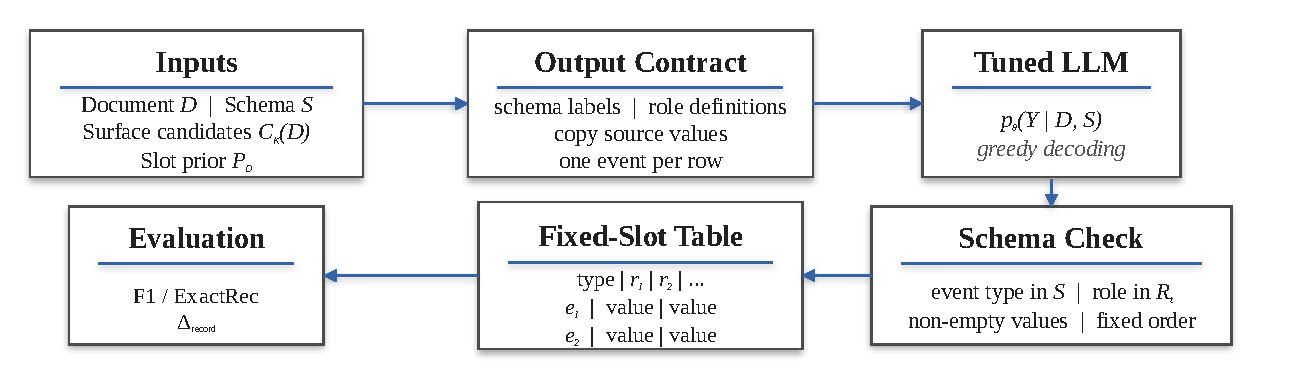
\includegraphics[width=\linewidth]{figures/fig2_gai.pdf}
\caption{Overview of \method. Document evidence, closed schemas, and optional prompt-level priors are rendered into a role-grounded output contract. An instruction-tuned LLM generates event rows, which are checked against the schema and normalized into fixed-slot records.}
\label{fig:sarge-pipeline}
\end{figure}

For each document, \method\ exposes the announcement text, closed schema, and source-grounding signals (Fig.~\ref{fig:sarge-pipeline}). The schema defines legal event types and role names, surface candidates emphasize copyable values, and an optional training-derived slot prior gives a coarse record-organization cue. An instruction-tuned model then generates event rows under deterministic decoding, after which the table is schema-checked and normalized into the benchmark fixed-slot representation.

This design separates schema closure from source grounding. Event types and roles are structural constraints that can be checked without gold answers, whereas document-visible values are evidence cues that encourage copying. Keeping this distinction explicit lets \method\ use candidates for grounding while still evaluating the model's own row construction.

The role-grounded instruction shifts the prediction unit from isolated arguments to event rows. The generator input is written as
\begin{equation}
x_D=\left[D;\mathcal{S};C_K(D);P_D;\mathcal{I}_{\mathcal{S}}\right],
\label{eq:prompt-interface}
\end{equation}
where $C_K(D)$ is a bounded surface-candidate set, $P_D$ is an optional slot-level prior, and $\mathcal{I}_{\mathcal{S}}$ requires exact schema labels and structured event rows. The reported $P_D$ is produced by a train-only prior planner from positive-count modes and role-fill frequencies; it never reads test gold event counts or gold active roles. $C_K(D)$ and $P_D$ are auxiliary prompt-level priors whose marginal utility is examined in the ablation analysis.

\paragraph{Prompt example (identical for SFT and inference).} \method\ sees one contract; only the answer block is supervised at training and generated at test:
{\scriptsize
\begin{verbatim}
[SCHEMA]  EquityPledge(Pledger, Pledgee, PledgedShares, StartDate)
[VALUES]  "Li", "Haitong", "1,188,600 shares", "2018-09-06", ...
[EVIDENCE]  <announcement D: a 2018-09-06 and an earlier 2017-12-07 pledge>
[TASK]  licensed types/roles only; copy source values; one event per row
[ANSWER]  {"events":[{"type":"EquityPledge","Pledger":"Li","Pledgee":
    "Haitong","PledgedShares":"1,188,600","StartDate":"2018-09-06"},
    {"type":"EquityPledge", ...}]}
\end{verbatim}}
Schema verification then filters unlicensed types or roles, removes empty fields, and maps valid rows to the fixed-slot table before evaluation.

\subsection{Surface-Value Grounding}

Financial announcements contain many values that should be copied rather than paraphrased. \method\ makes these strings explicit through surface-value grounding. The candidate pool is
\begin{equation}
C(D)=\{c_i=(s_i,b_i,e_i,\tau_i)\}_{i=1}^{N_D},
\label{eq:candidate-pool}
\end{equation}
where $s_i$ is a surface string, $(b_i,e_i)$ are its character offsets, and $\tau_i$ is a coarse surface type such as date, money, percentage, company name, or share quantity. Because long announcements contain many repeated or low-value strings, the prompt uses a bounded subset
\begin{equation}
C_K(D)=\operatorname{TopK}_{c_i\in C(D)}\phi(c_i,D,\mathcal{S}),
\label{eq:candidate-selection}
\end{equation}
where $\phi$ ranks candidates deterministically before rendering them in the prompt. Candidates are rule-extracted from the document text, deduplicated by string and offsets, and ordered by coarse type priority. The reported runs prioritize monetary values, share quantities, percentages, dates, full company names, person names, quoted entities, and stock codes; the main runs keep at most $K{=}20$ candidates with at most 6 per coarse type. Surface candidates only provide grounding cues; the event table is still generated by the role-grounded model.

\subsection{Role-Grounded Event-Table Generation}

Given $x_D$, \method\ generates a serialized event table $y=(y_1,\ldots,y_{|y|})$ under the standard autoregressive factorization. During supervised fine-tuning, the target sequence is the schema-valid serialization of the gold event table:
\begin{equation}
\mathcal{L}_{\mathrm{sft}}
=-\sum_{(D,Y_D^{\star})}\sum_{j=1}^{|y_D^{\star}|}
\log p_{\theta}(y_{D,j}^{\star}\mid x_D,y_{D,<j}^{\star}).
\label{eq:sft-loss}
\end{equation}
Only answer tokens contribute to this loss, so training aligns the model with the event-table output rather than with prompt reconstruction. At inference time, the main configuration uses greedy decoding over the tokenizer vocabulary, prioritizing stable schema labels and faithful value copying over diversity.

\subsection{Schema Checking and Fixed-Slot Normalization}

Generated rows are read from a structured event-row representation and retained when they satisfy schema closure. For a predicted row $\hat{e}$, validity is defined as
\begin{equation}
\operatorname{Valid}(\hat{e},\mathcal{S})
=\mathbf{1}[\hat{t}\in \mathcal{T}]\prod_{\hat{r}\in \operatorname{Keys}(\hat{e})}
\mathbf{1}[\hat{r}\in R_{\hat{t}}]\mathbf{1}[V_{\hat{r}}\neq\emptyset],
\label{eq:schema-validity}
\end{equation}
where $\hat{t}$ is the generated event type and $V_{\hat{r}}$ is the generated value set for role $\hat{r}$. This checks schema closure only: source grounding is encouraged by document-visible candidates and copy-oriented instructions, but is not a hard validation filter. The normalization procedure filters malformed rows, keeps schema-licensed types and roles, removes empty fields, normalizes role order, maps rows to the fixed-slot evaluator format, and removes duplicate argument strings within a role.

Valid rows are mapped to a fixed-slot table $Z_D=\{(t,\operatorname{slot}_{R_t}(\hat{e}))\mid \hat{e}\in\hat{Y}_D,\,\operatorname{Valid}(\hat{e},\mathcal{S})=1\}$. This normalization preserves dataset event types and role labels and places predictions in the benchmark event-table space. On the reported seed-13 runs, post-validation schema conformance is 100\% and there are zero parse failures, invalid event types, or invalid roles across both datasets, so the validity layer contributes no false positives to the recorded predictions.

\subsection{Record Organization Measure}

Schema-valid event rows support schema conformance but not exact record assembly. We evaluate this behavior with an exact-record measure. Records are normalized into role-to-value-set maps and aligned one-to-one within each document/event type by maximizing strict role-value overlap; ordinary groups use deterministic dynamic programming, while larger groups use linear assignment or deterministic greedy fallback. A pair is exact only when its two maps are identical, so any missing, extra, or wrongly assigned value makes the record non-exact:
\begin{equation}
\operatorname{ExactRec}=
\frac{2\sum_{D,t}\sum_{(e,\hat{e})\in\mathcal{M}_{D,t}}
\mathbf{1}[e=\hat{e}]}
{\sum_{D,t}\left(|Y_{D,t}|+|\hat{Y}_{D,t}|\right)}.
\label{eq:exact-record}
\end{equation}
We summarize the separation between F1 and exact-record performance as $\Delta_{\mathrm{record}}=\mathrm{F1}-\operatorname{ExactRec}$. This descriptive gap is not a pure binding-error estimate because ExactRec also penalizes missing, extra, or wrong values and event-count errors.

\section{Experiments}
\label{sec:experiments}

\subsection{Experimental Setup}

\textbf{Datasets.} We evaluate \method\ on ChFinAnn and DuEE-Fin \cite{han2022dueefin,zheng2019doc2edag}. ChFinAnn contains 32,040 Chinese financial announcements with five fixed event schemas; about 71\% of documents are single-event and 29\% are multi-event. DuEE-Fin contains 11,900 financial documents with a larger event and role inventory; about 67\% are single-event and 33\% are multi-event.

\textbf{Metrics.} Following prior Chinese financial DEE work \cite{chen2025docfee,han2022dueefin,zheng2019doc2edag}, F1 uses the Doc2EDAG fixed-schema event-table protocol: each predicted event selects a same-type gold event without replacement, and precision/recall/F1 are micro-averaged over matched role values. We report F1(S.) and F1(M.) on single- and multi-event subsets. ExactRec is the strict event-row match in Eq.~\ref{eq:exact-record}, and $\Delta_{\mathrm{record}}$ is F1--ExactRec.

\textbf{Implementation.} \method\ uses Qwen3-4B-Instruct-2507 as the base generator \cite{qwen3technical} with LoRA/QLoRA-style 4-bit NF4 fine-tuning \cite{dettmers2023qlora,hu2022lora}. Adapters use rank 16, $\alpha=32$, dropout 0.05, and $q/k/v/o$ projection modules; optimization uses learning rate $2{\times}10^{-4}$, two epochs, micro-batch size 1, gradient accumulation 8 (ChFinAnn seed 13) or 16 (DuEE-Fin, ChFinAnn seeds 17/42), and maximum sequence length 4096. Generation uses the compact prompt in \S\ref{sec:methodology}, maximum output length 1024, and greedy non-thinking decoding with one candidate per document. HF-4bit is the primary inference setting; vLLM-BF16 rows in the ablation table are backend sensitivity checks using merged-model serving \cite{kwon2023vllm}.

\textbf{Baselines.} We compare with representative document-level financial event extraction systems: Doc2EDAG, DE-PPN, PTPCG, GIT, ReDEE/RAAT, ProCNet, EPAL, and SEELE \cite{hu2025epal,liang2022raat,wang2023procnet,xu2021git,xu2024seele,yang2021deppn,zheng2019doc2edag,zhu2022ptpcg}.

\subsection{Main Results}

\begin{table}[t]
\centering
\caption{Main fixed-schema results. F1 follows the Doc2EDAG protocol; ExactRec is strict event-row match; $\Delta_{\mathrm{record}}$ is F1--ExactRec. Baseline ExactRec/$\Delta_{\mathrm{record}}$ are unavailable without prediction files. SEELE does not report F1(M.). $^{\dagger}$Doc2Event is contextual only: DuEE-Fin dev under its own scorer; F1 recomputed as 78.0 from P/R${=}80.7/75.5$; no ChFinAnn.}
\label{tab:main-results}
\scriptsize
\setlength{\tabcolsep}{2.6pt}
\resizebox{\ifdim\width>\linewidth \linewidth\else \width\fi}{!}{%
\begin{tabular}{@{}lrrrrrrrrrr@{}}
\toprule
Model & \multicolumn{5}{c}{ChFinAnn} & \multicolumn{5}{c}{DuEE-Fin} \\
\cmidrule(lr){2-6}\cmidrule(lr){7-11}
 & F1 & F1(S.) & F1(M.) & ExactRec & $\Delta_{\mathrm{record}}$ & F1 & F1(S.) & F1(M.) & ExactRec & $\Delta_{\mathrm{record}}$ \\
\midrule
Doc2EDAG~\cite{zheng2019doc2edag}    & 78.8 & 83.9 & 67.3 & -- & -- & 63.4 & 69.1 & 58.7 & -- & -- \\
DE-PPN~\cite{yang2021deppn}          & 79.9 & 85.9 & 68.4 & -- & -- & 45.1 & 54.2 & 21.8 & -- & -- \\
PTPCG~\cite{zhu2022ptpcg}            & 79.4 & 88.2 & --   & -- & -- & 66.0 & --   & --   & -- & -- \\
GIT~\cite{xu2021git}                 & 80.3 & 87.6 & 72.3 & -- & -- & 67.8 & 73.7 & 63.8 & -- & -- \\
ReDEE/RAAT~\cite{liang2022raat}      & 81.9 & 88.7 & 74.1 & -- & -- & 74.4 & 78.9 & 70.6 & -- & -- \\
ProCNet~\cite{wang2023procnet}       & 80.8 & 87.5 & 73.5 & -- & -- & 75.1 & 80.1 & 71.0 & -- & -- \\
EPAL~\cite{hu2025epal}               & 83.4 & 89.7 & 76.6 & -- & -- & 76.4 & 81.2 & 72.7 & -- & -- \\
SEELE~\cite{xu2024seele}             & 85.1 & --   & --   & -- & -- & 80.8 & --   & --   & -- & -- \\
Doc2Event~\cite{ding2025doc2event}$^{\dagger}$ & -- & -- & -- & -- & -- & 78.0 & 81.2 & 77.3 & -- & -- \\
\method\ (seed 13)                   & 86.0 & 89.9 & 81.8 & 58.4 & 27.6 & 78.0 & 79.3 & 77.5 & 42.8 & 35.2 \\
\method\ (mean, seeds 13/17/42)      & 85.6 & 89.2 & 81.7 & 56.1 & 29.5 & 78.3 & 79.8 & 77.6 & 43.3 & 35.1 \\
\method\ (std)                       & $\pm$0.4 & $\pm$0.7 & $\pm$0.1 & $\pm$2.0 & $\pm$1.6 & $\pm$0.4 & $\pm$0.5 & $\pm$0.2 & $\pm$0.5 & $\pm$0.1 \\
\bottomrule
\end{tabular}%
}
\end{table}

On ChFinAnn (Table~\ref{tab:main-results}), \method\ reaches $85.6\pm0.4$ F1, numerically above the listed baselines; on DuEE-Fin it reaches $78.3\pm0.4$ F1, below SEELE but above EPAL and ProCNet. The multi-event subset matters most: \method\ reaches $81.7\pm0.1$ F1(M.) on ChFinAnn, above directly comparable baselines that report it, and $77.6\pm0.2$ on DuEE-Fin, above EPAL and ProCNet. Doc2Event is contextual only because it uses a different split and scorer. Across both datasets ExactRec trails F1 by 29.5 and 35.1 points, making the role-to-exact-record discrepancy visible.

The seed-13 and mean rows indicate that the headline behavior is not a single-run artifact. ChFinAnn has standard deviation 0.4 F1 and 0.1 F1(M.), so the multi-event result is stable across seeds. DuEE-Fin is more competitive because SEELE remains stronger in aggregate F1, but \method\ still stays above EPAL and ProCNet and preserves a high multi-event score.

This record-level view clarifies the modeling difference: \method\ realizes value selection and row assignment within one output interface, whereas prior systems couple them through task-specific graph, query, probe, or structured-decoding modules. ExactRec makes the remaining assembly error explicit.

The gap should be read as a diagnostic rather than a contradiction of the F1 results. F1 rewards correct role values after event-level matching, so it captures whether the system has found the right financial facts. ExactRec asks the stricter question of whether all values belonging to one event row are jointly correct. Reporting both metrics therefore separates two practical requirements: extracting the right arguments and assembling them into evaluator-compatible records.

\subsection{Ablation Study}

\begin{table}[t]
\centering
\caption{Ablation grouped by factor. Rows use seed 13. Component rows isolate $C_K(D)$ and $P_D$; backend and decoding rows test inference sensitivity.}
\label{tab:ablation}
\scriptsize
\setlength{\tabcolsep}{2.6pt}
\resizebox{\ifdim\width>\linewidth \linewidth\else \width\fi}{!}{%
\begin{tabular}{@{}lrrrrrrrr@{}}
\toprule
Setting & \multicolumn{4}{c}{ChFinAnn} & \multicolumn{4}{c}{DuEE-Fin} \\
\cmidrule(lr){2-5}\cmidrule(lr){6-9}
 & F1 & ExactRec & $\Delta_{\mathrm{record}}$ & Path & F1 & ExactRec & $\Delta_{\mathrm{record}}$ & Path \\
\midrule
Same base, no SFT              & 24.8 & 10.2 & 14.6 & vLLM-BF16 & 3.3  & 0.0 & 3.3  & HF-4bit \\
\method\ (seed 13)             & 86.0 & 58.4 & 27.6 & HF-4bit   & 78.0 & 42.8 & 35.2 & HF-4bit \\
\,$-$ $C_K(D)$ (DuEE)          & --   & --   & --   & --        & 78.1 & 42.9 & 35.2 & HF-4bit \\
\,$-$ $P_D$ (DuEE)             & --   & --   & --   & --        & 77.6 & 42.9 & 34.7 & HF-4bit \\
\,$-$ $C_K(D)$ (ChFinAnn diag.)& 85.4 & 56.1 & 29.3 & vLLM-BF16 & --   & --   & --   & -- \\
\,$-$ $P_D$ (ChFinAnn diag.)   & 85.7 & 56.4 & 29.3 & vLLM-BF16 & --   & --   & --   & -- \\
vLLM-BF16 + LoRA $k_{\mathrm{cand}}{=}1$       & 85.5 & 55.9 & 29.5 & vLLM-BF16 & 75.0 & 38.2 & 36.8 & vLLM-BF16 \\
vLLM-BF16 + LoRA $k_{\mathrm{cand}}{=}4\,T{=}0.7$ & 84.2 & 55.0 & 29.3 & vLLM-BF16 & 73.1 & 34.7 & 38.4 & vLLM-BF16 \\
\bottomrule
\end{tabular}%
}
\end{table}

Table~\ref{tab:ablation} separates three factors. Removing supervised fine-tuning collapses F1 from 86.0 to 24.8 on ChFinAnn and from 78.0 to 3.3 on DuEE-Fin: the un-tuned model often emits schema-legal but empty or sparse rows, so the gain is alignment to the event-table interface rather than raw capacity. Under backend-matched comparisons, removing $C_K(D)$ or $P_D$ shifts F1 by at most 0.4 points and ExactRec by at most 0.5 points, suggesting weak cues rather than independently decisive modules. Switching from greedy single-candidate decoding to sampled four-candidate decoding ($k_{\mathrm{cand}}{=}4,T{=}0.7$) decreases F1 by 1.3 and 1.9 points on ChFinAnn and DuEE-Fin, respectively.

These ablations qualify the contribution. The surface-value and slot-prior cues make the prompt more informative, but the small deltas show that they are not hidden sources of gold information. The dominant factor is training the model to interpret the schema contract and emit evaluator-compatible rows. Sampling hurts because closed-schema extraction rewards one stable table more than diverse alternatives.

\paragraph{Case study.} In a ChFinAnn equity-pledge document, two gold records share pledger Li and pledgee Haitong but differ in private values: 1,188,600 shares on 2018-09-06 versus 12,151,000 shares on 2017-12-07. The base model without SFT emits one \texttt{EquityPledge} row with empty arguments; \method\ generates two schema-valid rows and separates the shared arguments from record-specific dates and share quantities. The new pledge is exact, but the earlier row copies 17,011,400 instead of 12,151,000, so record-level binding needs the correct private value per row, not merely plausible ones.

\subsection{Smaller-Backbone Evidence}

\begin{table}[t]
\centering
\caption{Smaller-backbone evidence on test splits. All rows use seed 13; these are not strict same-checkpoint scale controls.}
\label{tab:smaller-backbone}
\scriptsize
\setlength{\tabcolsep}{2.6pt}
\resizebox{\ifdim\width>\linewidth \linewidth\else \width\fi}{!}{%
\begin{tabular}{@{}lrrrrrrrr@{}}
\toprule
Setting & \multicolumn{4}{c}{ChFinAnn} & \multicolumn{4}{c}{DuEE-Fin} \\
\cmidrule(lr){2-5}\cmidrule(lr){6-9}
 & F1 & F1(M.) & ExactRec & $\Delta_{\mathrm{record}}$ & F1 & F1(M.) & ExactRec & $\Delta_{\mathrm{record}}$ \\
\midrule
Qwen3-4B + SFT/LoRA   & 86.0 & 81.8 & 58.4 & 27.6 & 78.0 & 77.5 & 42.8 & 35.2 \\
Qwen3-4B no SFT       & 24.8 & 6.8 & 10.2 & 14.6 & 3.3 & 3.0 & 0.0 & 3.3 \\
Qwen3-1.7B + SFT/LoRA & 83.9 & 79.6 & 52.8 & 31.1 & 64.6 & 65.4 & 26.5 & 38.1 \\
Qwen3-0.6B + SFT/LoRA & 82.2 & 74.4 & 48.8 & 33.4 & 60.6 & 56.9 & 20.2 & 40.4 \\
\bottomrule
\end{tabular}%
}
\end{table}

\begin{table}[t]
\centering
\caption{ChFinAnn multi-event robustness. \emph{S--M Gap} is F1(S.)--F1(M.); lower values indicate less degradation from single-event to multi-event documents. EPAL is the strongest published baseline among methods that report both F1(S.) and F1(M.).}
\label{tab:multievent}
\scriptsize
\setlength{\tabcolsep}{4pt}
\resizebox{\ifdim\width>\linewidth \linewidth\else \width\fi}{!}{%
\begin{tabular}{@{}lrrrr@{}}
\toprule
Method & F1 & F1(S.) & F1(M.) & S--M Gap \\
\midrule
EPAL~\cite{hu2025epal}              & 83.4 & 89.7 & 76.6 & 13.1 \\
Qwen3-1.7B + \method               & 83.9 & 87.8 & 79.6 & 8.2  \\
Qwen3-4B + \method (3-seed mean)   & 85.6 & 89.2 & 81.7 & 7.5  \\
\bottomrule
\end{tabular}%
}
\end{table}

Tables~\ref{tab:smaller-backbone} and~\ref{tab:multievent} separate supervised alignment from the strongest 4B configuration. On ChFinAnn, the 1.7B and 0.6B SFT runs substantially exceed the 4B no-SFT generator, and the 1.7B run already exceeds EPAL on multi-event F1 (79.6 vs.\ 76.6); on DuEE-Fin, the 1.7B SFT run is far above the no-SFT generator but below the 4B SFT run. The multi-event advantage is not unique to the 4B configuration, while DuEE-Fin remains more sensitive to backbone capacity and checkpoint differences.

\subsection{Efficiency}

\begin{table}[t]
\centering
\caption{Training-cost summary. \emph{Train} is wall-clock LoRA SFT time in minutes on a single 4090; \emph{Alloc.}\ and \emph{Resv.}\ are PyTorch CUDA peak allocated and reserved memory (GB). Batched inference throughput and per-request latency are reported in the text.}
\label{tab:efficiency}
\scriptsize
\setlength{\tabcolsep}{2.6pt}
\resizebox{\ifdim\width>\linewidth \linewidth\else \width\fi}{!}{%
\begin{tabular}{@{}lrrrrrr@{}}
\toprule
Backbone & \multicolumn{3}{c}{ChFinAnn} & \multicolumn{3}{c}{DuEE-Fin} \\
\cmidrule(lr){2-4}\cmidrule(lr){5-7}
 & Train & Alloc. & Resv. & Train & Alloc. & Resv. \\
\midrule
Qwen3-4B (3-seed) & $505.0\pm2.3$ & 12.5 & 22.9 & $165.8\pm1.6$ & 12.5 & 20.8 \\
Qwen3-1.7B & 302.1 & 10.4 & 20.2 & 82.2 & 10.4 & 22.4 \\
Qwen3-0.6B & 307.7 & 8.6 & 19.6 & 74.5 & 8.6 & 22.7 \\
\bottomrule
\end{tabular}%
}
\end{table}

Table~\ref{tab:efficiency} summarizes training cost across model scales; batched inference throughput and per-request latency are reported below. The three-seed 4B SFT runs take about 8.4 h on ChFinAnn and 2.8 h on DuEE-Fin at ${\sim}12.5$\,GB peak on a single 4090, and the 1.7B/0.6B runs are cheaper. Batched vLLM-BF16 test inference on the 1.7B and 0.6B models reaches 6.4--10.8 documents/s end to end (after pre-batching). A per-request profiler on the 0.6B DuEE-Fin model records p50/p95${=}1.82/5.67$\,s and 38.9 tokens/s; by prompt-length bucket p50 is 1.65/1.72/2.25\,s (short/medium/long), so length is a visible but not dominant cost factor at this scale.

\section{Limitations}
\label{sec:limitations}

Several scope conditions bound the reported results. \method\ uses a 4B generator while several baselines are smaller encoder-based systems, so the comparison evaluates the formulation rather than same-compute parity; the 1.7B/0.6B runs narrow this concern but are not strict same-checkpoint controls. External LLM-based DEE comparison is also limited: Doc2Event~\cite{ding2025doc2event} covers no ChFinAnn and releases no predictions for re-scoring under the same protocol. The largest open problem is record assembly itself: ExactRec trails F1 by about 30 and 35 points, so correct role values are still frequently assigned to imperfect rows. Efficiency metadata covers LoRA training time, peak memory, and batched throughput, but per-request latency is profiled only for the 0.6B DuEE-Fin configuration. Finally, checkpoint-family differences and Qwen3 pre-training are not separately controlled.

\section{Conclusion}
\label{sec:conclusion}

We began from a concrete obstacle in Chinese financial DEE: under shared evidence, correct role values are routinely assembled into the wrong event rows. \method\ addresses it by treating the fixed-slot event table as one schema-grounded prediction object, reaching F1 of 86.0 on ChFinAnn and 78.0 on DuEE-Fin. The payoff is largest exactly where the problem is hardest: on the multi-event subset it reaches 81.8 F1(M.) with the smallest single-to-multi degradation among comparable systems, and this advantage is already visible with a 1.7B backbone. The ExactRec/$\Delta_{\mathrm{record}}$ diagnostic turns the remaining record-assembly discrepancy into a measurable target, establishing homogeneous-record assembly as a distinct evaluation axis and marking the clearest next step for closing the gap this formulation opens.

\begin{credits}
\subsubsection{\ackname}
This work was supported in part by the National Key R\&D Program of China (2023YFC3305103 and 2023YFC3305102), and in part by the Heilongjiang Provincial Natural Science Foundation of China (No. ZD2025F003).

\subsubsection{\discintname}
The authors have no competing interests to declare.
\end{credits}

\bibliographystyle{splncs04}
\bibliography{references}

\end{document}
